\documentclass{beamer}
\mode<presentation>
\usepackage{amsmath}
\usepackage{amssymb}
%\usepackage{advdate}
\usepackage{adjustbox}
\usepackage{subcaption}
\usepackage{enumitem}
\usepackage{multicol}
\usepackage{mathtools}
\usepackage{listings}
\usepackage{xcolor}

\definecolor{mygray}{rgb}{0.5,0.5,0.5}
\definecolor{mymauve}{rgb}{0.58,0,0.82}
\definecolor{myblue}{rgb}{0.13,0.13,0.6}

\lstset{
	language=Python,
	backgroundcolor=\color{white},
	commentstyle=\color{mygray},
	keywordstyle=\color{myblue},
	numberstyle=\tiny\color{mygray},
	stringstyle=\color{mymauve},
	basicstyle=\ttfamily\small, % Change font size here
	breaklines=true,
	numbersep=8pt,
	showstringspaces=false,
	tabsize=4
}
\usepackage{url}
\def\UrlBreaks{\do\/\do-}
\usetheme{Boadilla}
\usecolortheme{lily}
\setbeamertemplate{footline}
{
  \leavevmode%
  \hbox{%
  \begin{beamercolorbox}[wd=\paperwidth,ht=2.25ex,dp=1ex,right]{author in head/foot}%
    \insertframenumber{} / \inserttotalframenumber\hspace*{2ex} 
  \end{beamercolorbox}}%
  \vskip0pt%
}
\setbeamertemplate{navigation symbols}{}

\providecommand{\nCr}[2]{\,^{#1}C_{#2}} % nCr
\providecommand{\nPr}[2]{\,^{#1}P_{#2}} % nPr
\providecommand{\mbf}{\mathbf}
\providecommand{\pr}[1]{\ensuremath{\Pr\left(#1\right)}}
\providecommand{\qfunc}[1]{\ensuremath{Q\left(#1\right)}}
\providecommand{\sbrak}[1]{\ensuremath{{}\left[#1\right]}}
\providecommand{\lsbrak}[1]{\ensuremath{{}\left[#1\right.}}
\providecommand{\rsbrak}[1]{\ensuremath{{}\left.#1\right]}}
\providecommand{\brak}[1]{\ensuremath{\left(#1\right)}}
\providecommand{\lbrak}[1]{\ensuremath{\left(#1\right.}}
\providecommand{\rbrak}[1]{\ensuremath{\left.#1\right)}}
\providecommand{\cbrak}[1]{\ensuremath{\left\{#1\right\}}}
\providecommand{\lcbrak}[1]{\ensuremath{\left\{#1\right.}}
\providecommand{\rcbrak}[1]{\ensuremath{\left.#1\right\}}}
\theoremstyle{remark}
\newtheorem{rem}{Remark}
\newcommand{\sgn}{\mathop{\mathrm{sgn}}}
\providecommand{\abs}[1]{\left\vert#1\right\vert}
\providecommand{\res}[1]{\Res\displaylimits_{#1}} 
\providecommand{\norm}[1]{\lVert#1\rVert}
\providecommand{\mtx}[1]{\mathbf{#1}}
\providecommand{\mean}[1]{E\left[ #1 \right]}
\providecommand{\fourier}{\overset{\mathcal{F}}{ \rightleftharpoons}}
%\providecommand{\hilbert}{\overset{\mathcal{H}}{ \rightleftharpoons}}
\providecommand{\system}{\overset{\mathcal{H}}{ \longleftrightarrow}}
	%\newcommand{\solution}[2]{\textbf{Solution:}{#1}}
%\newcommand{\solution}{\noindent \textbf{Solution: }}
\providecommand{\dec}[2]{\ensuremath{\overset{#1}{\underset{#2}{\gtrless}}}}
\newcommand{\myvec}[1]{\ensuremath{\begin{pmatrix}#1\end{pmatrix}}}
\newcommand{\mydec}[1]{\ensuremath{\begin{vmatrix}#1\end{vmatrix}}}
\let\vec\mathbf

\lstset{
%language=C,
frame=single, 
breaklines=true,
columns=fullflexible
}

\numberwithin{equation}{section}

\title{Affine Transformations}
\author{Y Siddhanth \\ EE24BTECH11059\\ EE1030}

\date{\today} 
\begin{document}

\begin{frame}
\titlepage
\end{frame}

\section*{Outline}
\begin{frame}
\tableofcontents
\end{frame}
\section{Problem}
\begin{frame}
\frametitle{Problem Statement}
Plot the ellipse whose focus is $\myvec{1 \\ -1}$, directrix $x-y-3 = 0$, and $e = \frac{1}{2}$. Plot the corresponding standard ellipse in the same graph using Affine Transformation.
\end{frame}

\section{Solution}
\subsection{Information Table}
%\begin{frame}
%\frametitle{Information Table}
	%\begin{table}[h!]    
		%\centering
		%

	%\end{table}
%\end{frame}
\subsection{Method of Solving}
\begin{frame}
	\frametitle{Method of Solving}
First we find the second order equation of the actual ellipse using the eccentricity definition.\\Let \(P\myvec{x\\y}\) be any point on the ellipse and PM be the perpendicular from P on the directrix. Then,
\begin{align}
	FP &= e \times PM\\
	FP &= \frac{1}{2} \times PM\\
	2FP &= PM\\
	4(FP)^2 &= PM^2\\
	4\sbrak{\brak{x+1}^2 + \brak{y-1}^2} &= \brak{\frac{x - y + 3}{\sqrt{1^2 + (-1)^2}}}^2\\
	4\sbrak{\brak{x+1}^2 + \brak{y-1}^2}  &= \brak{\frac{x - y + 3}{\sqrt{2}}}^2
\end{align}
\end{frame}
\begin{frame}
	\frametitle{Method of Solving}
	Upon simplification, we get the second order two variable conic equation to be,
	\begin{align}
		\frac{7}{4}\brak{x^2+y^2} + \frac{1}{2}xy + \frac{5}{2}\brak{-x+y} + \frac{7}{4} = 0 \label{acconiceq}
	\end{align}
	Comparing \eqref{acconiceq} with $x^\top\vec{V}x + 2\vec{u}^\top x + f = 0$, we get:
	\begin{align}
		\vec{V} &= \myvec{\frac{7}{4} & \frac{1}{4} \\ \frac{1}{4} & \frac{7}{4}} ,
		\\
		\vec{u} &=\frac{5}{4}  \myvec{ -1 \\ 1}
		\\
		f &= \frac{7}{4}
	\end{align}
\end{frame}
\begin{frame}
	\frametitle{Method of Solving}
	For Affine Transformation, we have to spectral / eigen decompose the matrix $\vec{V}$. \\ 
	\begin{align}
		\vec{V} = \vec{P}\vec{D}\vec{P^\top}
	\end{align}
	To find $\vec{D}$, we will have to find the eigen values of the matrix $\vec{V}$.
	\begin{align}
		|\vec{V}  - \lambda\vec{I}|  &= 0,\\
		|\vec{V}  - \lambda\vec{I}|  &= \begin{bmatrix}\frac{7}{4} - \lambda& \frac{1}{4}\\ \frac{1}{4} & \frac{7}{4} - \lambda\end{bmatrix}\\
		\lambda_1, \lambda_2 &= \frac{3}{2} , 2\\
		\therefore 	\vec{D} &= \myvec{\frac{3}{2} & 0 \\ 0 & 2	} \label{Ddef}
	\end{align}
\end{frame}
\begin{frame}
	\frametitle{Method of Solving}
	Note: In \eqref{Ddef}, the order of the eigen values that I have chosen is from smallest to biggest due to eccentricity calculation.\\
	\\
	Now, to find $\vec{P}$ which is the matrix containing the normalized eigen vectors. So we have to find the eigen-values.
	\begin{align}
		\vec{V}\vec{p_1^\prime} &= \lambda_1 \vec{p_1^\prime} \\
		\myvec{\frac{7}{4} & \frac{1}{4} \\ \frac{1}{4} & \frac{7}{4}} \vec{p_1^\prime}  &= \frac{3}{2}\vec{p_1^\prime} \\
	\end{align}
	Taking an augmented matrix,
	\begin{align}
		\brak{
			\begin{array}{cc|c}
				\frac{7}{4} - \lambda_1 & \frac{1}{4} & 0\\ 
				\frac{1}{4} & \frac{7}{4} - \lambda_1& 0
		\end{array}}\vec{p_1^\prime} 
	\end{align}
\end{frame}
\begin{frame}
	\frametitle{Method of Solving}
	\begin{align}
		\brak{
			\begin{array}{cc|c}
				\frac{1}{4} & \frac{1}{4} & \frac{3}{2}\\ 
				\frac{1}{4} & \frac{1}{4} & \frac{3}{2}
		\end{array}}
		\xleftrightarrow[]{R_1 \leftarrow {4 R_1}}
		\xleftrightarrow[]{R_2 \leftarrow {R_2-\frac{1}{4}R_1}}
		\brak{
			\begin{array}{cc|c}
				1 & 1 & 0\\ 
				0 & 0 & 0
		\end{array}}
	\end{align}
	If we take $\vec{p_1^\prime}  = \myvec{p_{11}^\prime \\ p_{12}^\prime}$, and put in the above equation, we get,
	\begin{align}
		\vec{p_1^\prime} = p_{11}^\prime \myvec{-1 \\ 1} \implies \vec{p_1^\prime} =  \myvec{-1 \\ 1}
	\end{align}
	$\therefore \vec{p_1^\prime}  = \myvec{-1 \\ 1} \implies \vec{p_1} = \frac{\vec{p_1^\prime} }{\norm{\vec{p_1^\prime}}}  = \myvec{ -\frac{1}{\sqrt{2}} \\ \frac{1}{\sqrt{2}}}$ \\
\end{frame}
\begin{frame}
	\frametitle{Method of Solving}
	Similarly solving for $\vec{p_2^\prime}$ , we get,
	\begin{align}
		\vec{p_2^\prime} &=  \myvec{1 \\ 1} \\
	\end{align} 
	$\therefore \vec{p_2^\prime}  = \myvec{1 \\ 1} \implies \vec{p_2} = \frac{\vec{p_2^\prime} }{\norm{\vec{p_2^\prime}}}  = \myvec{ \frac{1}{\sqrt{2}} \\ \frac{1}{\sqrt{2}}}$ \\
	By definition $\vec{P} = \sbrak{\vec{p_1} ~ \vec{p_2}}$ \\ 
	
	\begin{align}
		\vec{P} = \myvec{ - \frac{1}{\sqrt{2}} & \frac{1}{\sqrt{2}} \\ \frac{1}{\sqrt{2}} & \frac{1}{\sqrt{2}} } \label{Rdef}
	\end{align}
	By comparing $\vec{P}$ with a standard rotation matrix, $\myvec{\cos\theta & -\sin\theta \\ \sin\theta & \cos\theta}$
	the angle of rotation of $\vec{P}$ is $\arccos\brak{- \frac{1}{\sqrt{2}}}$ or $\frac{3\pi}{4}$. \\\\
\end{frame}
\subsection{Affine Transformation}
\begin{frame}
	\frametitle{Affine Transformation}
	Now, we will use Affine Transformations to get the standard ellipse equation.
	
	\begin{align}
		\vec{y}^\text{T}\brak{\frac{\vec{D}}{f_0}}\vec{y} &= 1\\
		\vec{x} &= \vec{Py} + \vec{c} \label{t1}\\
	\end{align}
	
	Where 
	
	\begin{align}
		f_0 &= \vec{u}^\text{T}\vec{V}^{-1}\vec{u} - f  = \frac{25}{4} \myvec{-1 & 1} \myvec{\frac{7}{12} & \frac{-1}{12} \\ \frac{-1}{12} & \frac{7}{12}}  \myvec{-1 \\ 1}  - \frac{7}{4}= \frac{25}{12} -  \frac{7}{4} = \frac{1}{3}\\
		\vec{c} &= -\vec{V}^{-1}\vec{u} = -\frac{5}{4}  \myvec{-1 & 1} \myvec{\frac{7}{12} & \frac{-1}{12} \\ \frac{-1}{12} & \frac{7}{12}}\myvec{ -1 \\ 1} = \frac{5}{6}  \myvec{ 1 \\ -1}
	\end{align}
\end{frame}
\begin{frame}
	\frametitle{Affine Transformation}
	Finally, we get the standard form of the ellipse.
	
	\begin{align}
		\vec{y}^\text{T}\myvec{\frac{3}{2} & 0 \\ 0 & 2}\vec{y} &= \frac{1}{3}
	\end{align}
	Plotting the standard and the actual ellipse using python,
	
	\begin{figure}[H]
		\centering
		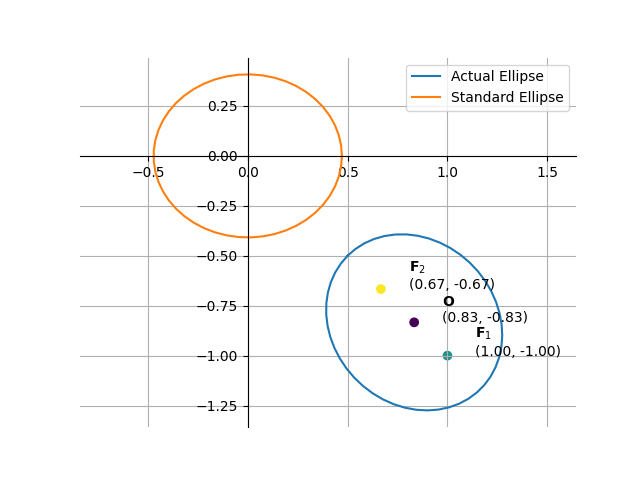
\includegraphics[width=0.7\columnwidth]{figs/fig1.png} 
		\caption{}
		\label{fig1}
	\end{figure} 
\end{frame}
\begin{frame}
	\frametitle{Affine Transformation}
To find the lengths of the semi-major and semi-minor axis, 
	\begin{align}
		a &= \sqrt{\brak{\frac{f_0}{\lambda_1}}} =  \sqrt{\frac{2}{9}}\\
		b &= \sqrt{\brak{\frac{f_0}{\lambda_2}}} = \sqrt{\frac{1}{6}}
	\end{align}
	Equations of the minor and major axis of the actual ellispe can be found with $p_i(x - c) = 0$, $i = 1, 2$ respectively \\ 
	\begin{align}
		\text{Minor Axis} \equiv   \myvec{- \frac{1}{\sqrt{2}} & \frac{1}{\sqrt{2}}}x = 0\\
		\text{Major Axis} \equiv   \myvec{\frac{1}{\sqrt{2}} & \frac{1}{\sqrt{2}}}x = 0
	\end{align}
	The Latus rectum of the ellipse can be found with,
	\begin{align}
		l = 2\frac{\sqrt{|f_0 \lambda_1|}}{\lambda_2} = \frac{1}{\sqrt{2}}
	\end{align}
\end{frame}

\end{document}
